\chapter[Targeted Optimisation of Atomic Networks]{Targeted Optimisation of \\ Atomic Networks}
\label{ch:targetedopt}

\begin{chapterabstract}
A targeted optimisation method is presented which enables \td{} networks to be constructed by reference to a set of ring statistics and \aw{} parameter, $\alpha$, which controls the preferred nearest\--neighbour spatial correlations.
The method efficiently utilises the dual lattice and allows systematic exploration of configurational space. 
Three different systems are considered; a system containing 5\--, 6\-- and 7\--membered rings only (a proxy for amorphous graphene), the configuration proposed by Zachariasen, and those
observed experimentally for ultra\--thin films of \sioii. 
The system energies are investigated as a function of the network topologies and the range of physically\--realisable structures established and compared to known experimental results.
The limits on $\alpha$ are evaluated, whilst the evolution of the network structure as a function of topology is discussed in terms of the ring\--ring pair distribution functions.
A short study on ring percolation in amorphous graphene is also presented.
\end{chapterabstract}


\section{Disorder in Two\--Dimensional Networks}

A central theme in this thesis is that the characterisation of the disorder in \td{} networks can be achieved through the ring structure. 
For 3\--coordinate atomic materials the mean ring size is constrained to six by Euler's law, which allows the variance of the ring size distribution, $\mu_2$, to act as a proxy measure for disorder (see sections \ref{s:eulerslaw} and \ref{s:lemaitre}).
The same set of ring statistics can however lead to a large number of different ring arrangements, as shown in figure \ref{fig:zach}.
These can be further quantified by the \aw{} parameter, $\alpha$, which measures the ring\--ring correlations.
An interesting observation across a wide range of experimental systems is that the measured value of the \aw{} parameter lies in a tight range of $\alpha\approx0.15\rightarrow 0.3$ \cite{Zsoldos1999}.
This effect is also seen in computational studies, including for example the previous chapter.

Whilst it is necessary for good computational models to capture these measures accurately, they do not give insight into \textit{why} such configurations are preferred. 
To answer this question a different approach is required, where configurations can be systematically generated, covering a parameter space which extends beyond the experimentally accessible region.
To achieve this a targeted optimisation method can be employed, whereby configurations are produced to fit network properties, and not driven by an underlying potential model.
This allows the experimentally occurring structures to be viewed in the context of the wider configurational landscape.

\section{Targeted Optimisation Algorithm}
\label{s:targetedoptalg}

The primary remit of the targeted optimisation algorithm is to generate plausible network configurations based on the supplied network properties of ring statistics and \aw{} parameter.
A secondary requirement is for the method to be efficient enough to produce samples for further high throughput calculations.
Both of these goals can be successfully accomplished with the method presented here: a \mc{} search algorithm, using the machinery of bond switching.

The bond switching algorithm (described in detail in section \ref{s:bondswitch}), amorphises a crystalline hexagonal lattice by exchanging the neighbouring interactions between pairs of bonded atoms and geometry optimising the structure.
Moves are accepted according to the resulting change in the potential energy, where those with lower energy are accepted with increasing probability.
The driving force is therefore always towards a structure which is physically motivated.
In targeted optimisation, the same Monte Carlo moves are proposed as in bond switching, but crucially moves are not accepted on the basis of the energy of the network, but rather its agreement with a target ring distribution and \aw{} parameter.
This agreement is measured by a cost function of the form:
\begin{equation}
	\label{eq:costfunc}
	\obj=\fk_\alpha\abs{\alpha-\alpha^t}+\frac{\abs{\mu_2-\mu_2^t}}{\mu_2^t}+\sumk\frac{\abs{p_k-p_k^t}}{p_k^t},
\end{equation} 
where $\fk_\alpha$ is a scaling constant; $p_k^t$, $\mu_2^t$ and $\alpha^t$ are the input target values; $p_k$ are the system ring statistics; and $\mu_2$ and $\alpha$ are calculated from an \aw{} fit on the current state.
In the cost function the relative difference is used for the ring distribution, as the same accuracy is required for all $p_k^t$, which may differ by several orders of magnitude. 
This is not a concern for $\alpha^t$, which must also have the flexibility to take a zero value, and hence the absolute difference is used in the first term. 

Moves in targeted optimisation are accepted with probability given by the Metropolis condition:
\begin{equation}
	P_{ij}=\min\left[1,\exp{-\Delta\obj/T}\right]\,,
\end{equation}
where $\Delta\obj$ is the difference in cost functions before and after the proposed move, and $T$ is a temperature parameter. 
In contrast to bond switching which is concerned with sampling, this is a global optimisation algorithm and moves are proposed until the network has converged to the target properties and the cost function is zero.
As is the case with such optimisation techniques, steps must be taken to avoid becoming trapped in local minima. %, and the calculation not converging. 
This is achieved through selection of the parameters $\fk_\alpha$ and $T$. 
The parameter $\fk_\alpha$ changes the relative costs of satisfying the $\alpha^t$ and $p_k^t$ conditions, and must be chosen so that neither is overweighted. The parameter $T$ controls the proportion of moves which are accepted. 
Some temperature is required to overcome local minima, but if set too high the algorithm will no longer move downhill in cost %and the search becomes effectively random 
\-- invariably leading to non\--convergence. 
Values for $\fk_\alpha$ and $T$ can be determined from a parameter search checking for convergence of target systems; but $\fk_\alpha=10$ and $T\sim 10^{-4}$ were appropriate for systems of the type and size described in this work. 

One key point which arises from using a cost function is that there is no requirement for accurate on\--the\--fly geometry optimisation of the atomic positions (as there is no need to calculate potential energies).
It is the underlying topology of the network which determines the system properties, which is invariant to the geometry.
The final energy of the system may well be of interest, but this can be evaluated just once at the end of the calculation.
This opens the door for significant speed\--ups through efficient use of the dual lattice.

\subsection{Dual Space Implementation}

Whilst the targeted optimisation algorithm can be employed using atomic positions, there are significant advantages to a dual space implementation.
As discussed in section \ref{s:atomringnetworks}, the ring structure is better described through the use of the dual network. 
In this representation the ring statistics in equation \eqref{eq:costfunc} are simply given by the node degree distribution. 
In addition, the mean ring sizes about each ring, $m_j$, required for the Aboav\--Weaire fit (equation \eqref{eq:aboavweaire}) can be easily calculated from the joint degree distribution:
\begin{equation}
	\label{eq:mjejklink}
	m_j = \sumk \frac{ke_{jk}}{q_j}.
\end{equation}
Hence, by utilising the ring network, the book\--keeping to track the network properties is greatly simplified.

\begin{figure}[bt]
     \centering
     
     \begin{subfigure}[b]{0.3\textwidth}
         \centering
         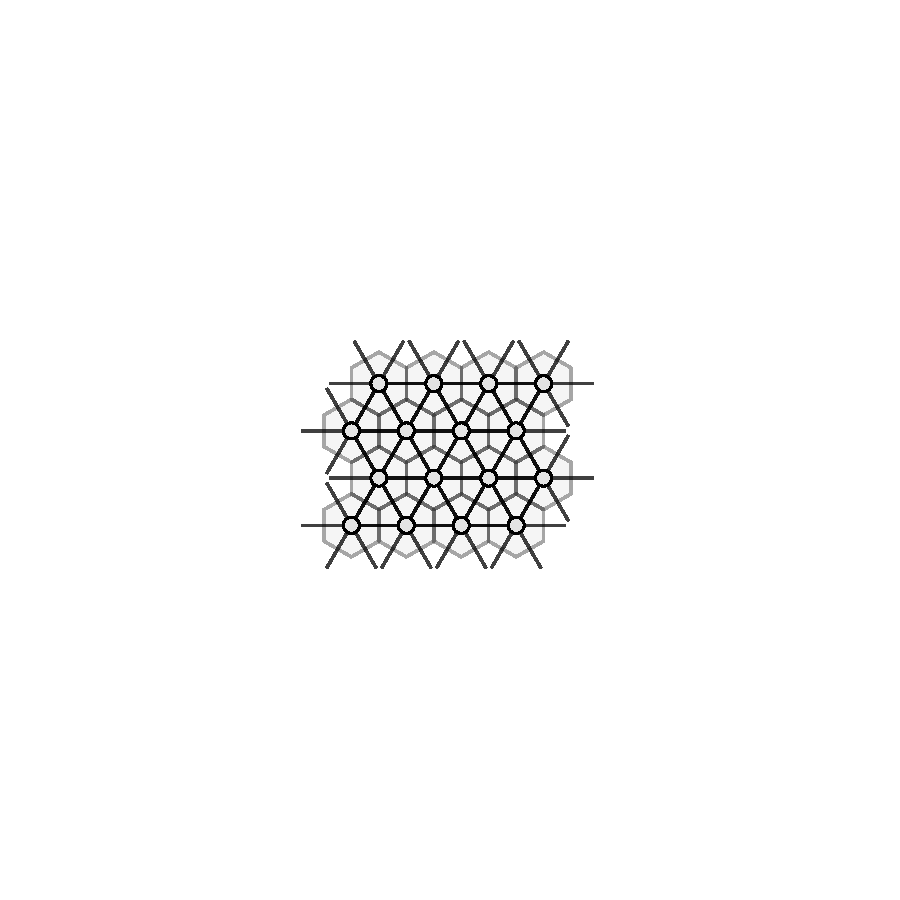
\includegraphics[height=3cm]{./figures/targeted_opt/dualswitch_0.pdf}
         \caption{}
         \label{fig:dualswitch1}
     \end{subfigure}
     \hfill
	\begin{subfigure}[b]{0.3\textwidth}
         \centering
         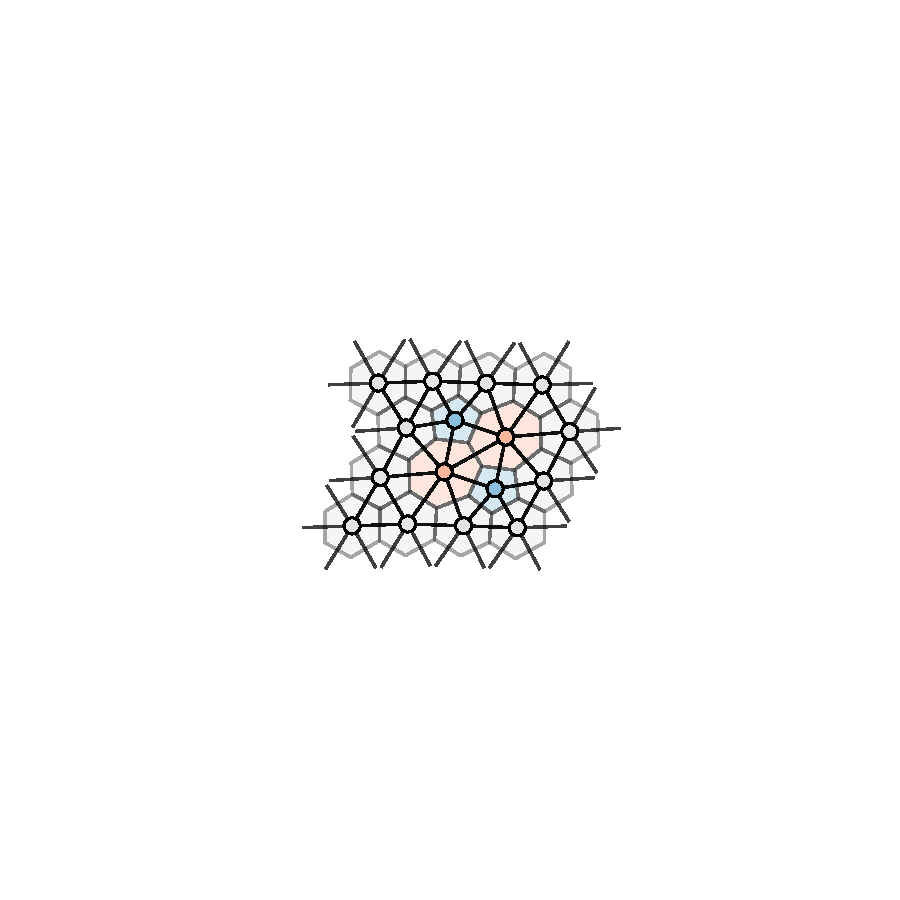
\includegraphics[height=3cm]{./figures/targeted_opt/dualswitch_1.pdf}
         \caption{}
         \label{fig:dualswitch2}
     \end{subfigure}
     \hfill
     \begin{subfigure}[b]{0.3\textwidth}
         \centering
         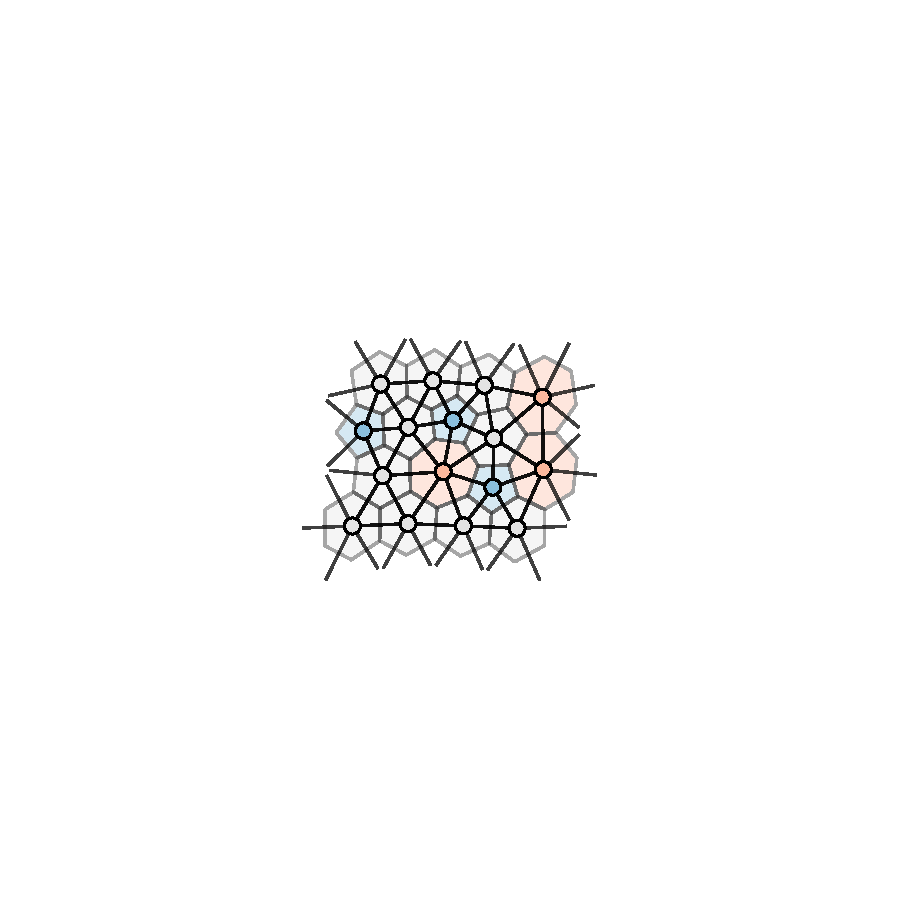
\includegraphics[height=3cm]{./figures/targeted_opt/dualswitch_2.pdf}
         \caption{}
         \label{fig:dualswitch3}
     \end{subfigure}

     \caption{Bond switching \mc{} moves can be performed solely through the dual lattice. Two successive moves are shown from (a)$\rightarrow$(b) and (b)$\rightarrow$(c). In the dual lattice (bold circles and lines) two edge\--sharing triangles are selected and the shared edge transposed. The atomic network is also shown (faded rings) to illustrate the corresponding effect on the atomic structure.}
     \label{fig:dualswitch}
\end{figure}

The implementation of the bond switching move itself is also straightforward in dual space.
Figure \ref{fig:dualswitch} shows how an atomic system can be manipulated \textit{solely} through the dual lattice.
Here the triangular nature of the dual (itself reflective of the trivalency of the atoms) can be exploited to good effect.
By selecting edge sharing triangles in the ring network and transposing the shared edge connection, a perturbation equivalent to the Stone\--Wales defect can be enacted. 
This process can be continued to generate an amorphous network. 

In addition, although there is no strict requirement for geometry optimisation after each step, the triangle lattice can be used to maintain a reasonable physical structure in a cost efficient manner.
By applying a harmonic potential, equation \eqref{eq:harmonic}, between all pairs of linked nodes, the ring centroids can be maintained at a reasonable separation.
The atomic positions can then be regenerated by reversing the triangulation, placing species at the centre of each triangle, relatively close to the minimum in the atomic potential energy surface.
Specifically, in this chapter a Keating potential, equation \eqref{eq:keating}, is used  with an interatomic separation of $r_0$ and $\fk_S=5\fk_A$ (as in previous studies of amorphous graphene \cite{Kumar2012}).
If the resultant polygons are assumed to be regular, the equilibrium separation for two polygons in the dual of sizes, $k_i$ and $k_j$, can be expressed:
\begin{equation}
	r_{ij}^0 = \frac{r_0}{2}\left(\frac{1}{\tan\left(\pi/k_i\right)}+\frac{1}{\tan\left(\pi/k_j\right)}\right).
\end{equation}
The extreme computational efficiency of evaluating the forces of the harmonic potential enables the targeted optimisation algorithm to complete rapidly whilst retaining the essential physics of the system.
The final geometry can then be refined.

\section{Mapping Configurational Space}
\label{s:toptmapconfigspace}

The targeted optimisation algorithm provides a opportunity to gain insight into the physical meaning of the \aw{} and its effect on network topology.
For this, a variety of test systems are used, the principle of which contains only $5\rightarrow 7$ membered rings.
This can be considered a proxy for amorphous graphene, aG,
%This system 
 and represents a useful framework for investigating the \aw{} law due to the presence of additional constraints which make it highly controllable. As a consequence of Euler's law the proportion of $5$\-- and $7$\-- rings must be equal, which leads to a trivial relationship between the second moment and proportion of $6$\--rings,
\begin{equation}
\label{eq:agcon}
        p_5=p_7=\frac{1}{2}\left(1-p_6\right), \qquad \mu_2=1-p_6.
\end{equation}
In addition, this allows the $\alpha$ parameter to be explicitly defined in terms of the difference between the 5\--5 and 5\--7 ring adjacencies:
\begin{equation}
	\label{eq:agalpha}
	\alpha = \frac{12\chi_{75}^5-\left(1-p_6\right)^2}{6\left(1-p_6\right)},
\end{equation}
where $\chi_{75}^5=e_{57}-e_{55}$ (details of the derivation can be found in appendix \ref{app:derivag}).
This makes the aG model the first example of a system where the $\alpha$ parameter is well defined in terms of the underlying ring structure.
It also highlights the relative complexity encoded in the \aw{} parameter for even a seemingly simple case.

Two further systems with fixed ring statistics are also used to provide supplementary results.
These are based on the \zach{} configuration \cite{Zachariasen1932}, figure \ref{fig:zach}, and experimental samples of silica glass \cite{Lichtenstein2012}, which are chosen to provide examples of increasing ring diversity, with the \zach{} sample containing ring sizes in the range $k=4\rightarrow 8$ and silica $k=4\rightarrow 10$. 
The ring distributions for all the systems used in this chapter are summarised in table \ref{tab:toptpk}.
In addition whereas the silica distribution should be easily achievable by the targeted optimisation algorithm (essentially following \lm's maximum entropy distribution), the \zach{} distribution provides a more ``extreme'' case, where the distribution is not unimodal and the proportion of $5$-rings is greatest.

%\begin{table}[h]
%	\centering
%	\caption{Ring statistics for systems used with the targeted optimisation algorithm.}
%	\label{tab:toptpk}
%	\begin{tabular}{c c c c}
%	\toprule
%	& aG & Zach. & \sioii \\[0.5mm]
%	\midrule
%	$p_4$ & - & $0.1$ & $0.040$ \\ 
%	$p_5$ & $\left(1-p_6\right)/2$ & $0.35$ & $0.268$ \\
%	$p_6$ & $p_6$ & $0.15$ & $0.420$ \\
%	$p_7$ & $\left(1-p_6\right)/2$ & $0.25$ & $0.210$ \\
%	$p_8$ & - & $0.15$ & $0.050$ \\
%	$p_9$ & - & - & $0.010$ \\
%	$p_{10}$ & - & - & $0.002$ \\
%	\bottomrule	
%	\end{tabular}
%\end{table}

\begin{table}[h]
	\centering
	\caption{Ring statistics for systems used with the targeted optimisation algorithm.}
	\label{tab:toptpk}
	\begin{tabular}{c c c c c c c c}
	\toprule
	& $p_4$ & $p_5$ & $p_6$ & $p_7$ & $p_8$ & $p_9$ & $p_{10}$ \\[0.5mm]
	\midrule
	aG &- & $\left(1-p_6\right)/2$ & $p_6$ & $\left(1-p_6\right)/2$ & - & - & -  \\	
	Zach. \cite{Zachariasen1932} & $0.10$ & $0.35$ & $0.15$ &  $0.25$ & $0.15$ & - & - \\	
	\sioii{} \cite{Lichtenstein2012} & $0.040$ & $0.268$ & $0.420$ & $0.210$ & $0.050$  & $0.010$ & $0.002$ \\
	\bottomrule	
	\end{tabular}
\end{table}

\subsection{Limits of the \aw{} Parameter}

To begin mapping the configurational space of these atomic networks, the range of accessible $\alpha$ values for the aG system can be determined by generating periodic networks containing $10^5$ rings with $0.1\leq p_6 \leq 0.9$. 
The aim of these simulations is to try and probe the topological limits of $\alpha$, and so a high number of \mc{} steps can be used, $10^{9}$, without the need for geometry optimisation.
Visualisations of the output of the targeted optimisation algorithm are given in figure \ref{fig:toptconfigs}, for $p_6=0.4$ and $\alpha=-0.3\rightarrow 0.3$.
These images give a good qualitative feel for the physical meaning of the \aw{} parameter: at low $\alpha$ similar sized rings tightly cluster together, dispersing as $\alpha$ increases to favour dissimilar ring pairings.
Figure \ref{fig:alphalim} shows the range of accessible $\alpha$ values
as a function of $p_6$ \ie{} those for which the targeted optimisation algorithm converges.
The upper limit, $\alpha_{\mathrm{max}}$, appears a relatively weak function of $p_6$ whilst the lower limit, $\alpha_{\mathrm{min}}$, shows a much
stronger dependence.
In addition, the range of accessible values, $\Delta\alpha=\alpha_{\mathrm{max}}-\alpha_{\mathrm{min}}$, broadly mirrors the system entropy, although there is deviation around $p_6=1/3$.

\begin{figure}[bt]
     \centering
     
     \begin{subfigure}[b]{0.45\textwidth}
         \centering
         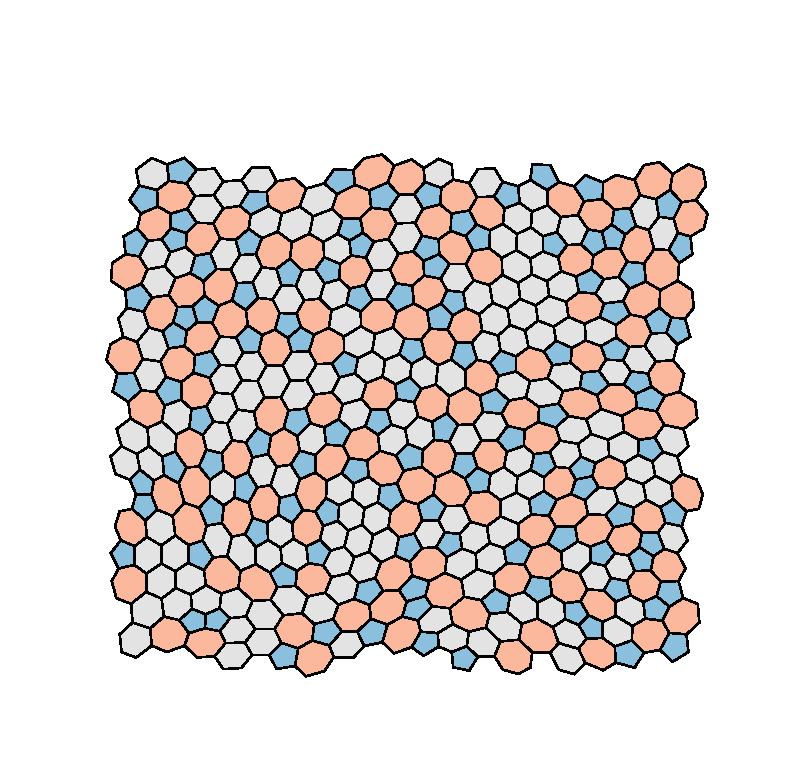
\includegraphics[width=0.9\textwidth]{./figures/targeted_opt/topt_30.pdf}
         \caption{$p_6=0.4$, $\alpha=0.3$}
         \label{fig:toptconfigs1}
     \end{subfigure}
     \hfill
     \begin{subfigure}[b]{0.45\textwidth}
         \centering
         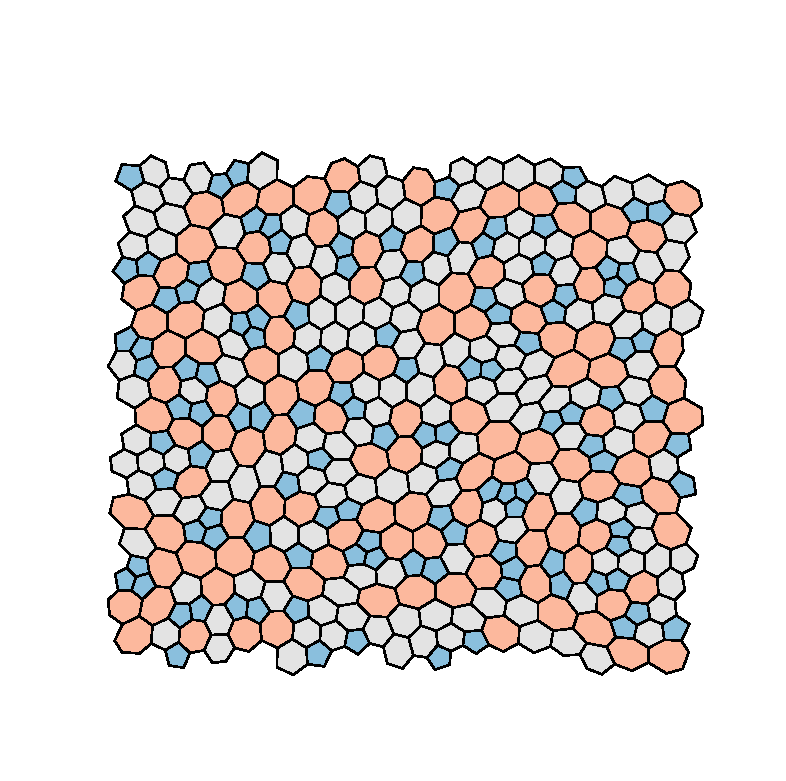
\includegraphics[width=0.9\textwidth]{./figures/targeted_opt/topt_10.pdf}
         \caption{$p_6=0.4$, $\alpha=0.1$}
         \label{fig:toptconfigs2}
     \end{subfigure}
     
     \vspace{2mm}
     \begin{subfigure}[b]{0.45\textwidth}
         \centering
         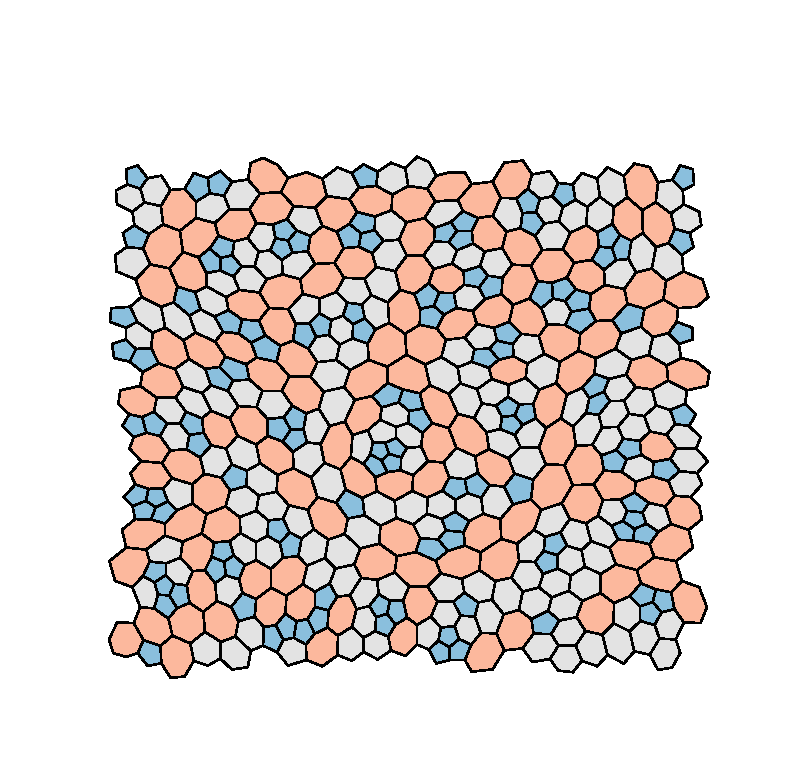
\includegraphics[width=0.9\textwidth]{./figures/targeted_opt/topt_-10.pdf}
         \caption{$p_6=0.4$, $\alpha=-0.1$}
         \label{fig:toptconfigs3}
     \end{subfigure}
     \hfill
     \begin{subfigure}[b]{0.45\textwidth}
         \centering
         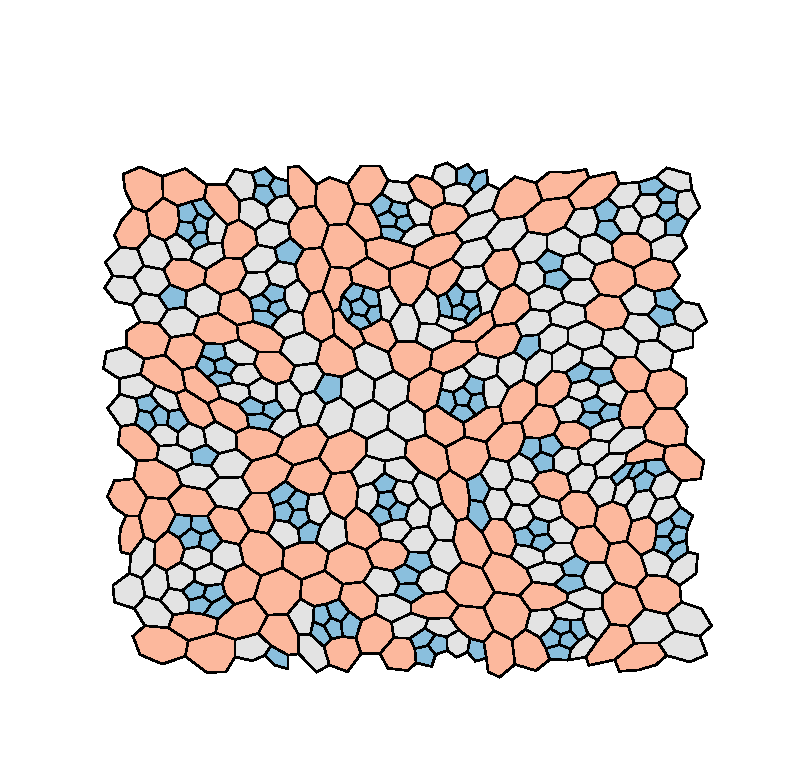
\includegraphics[width=0.9\textwidth]{./figures/targeted_opt/topt_-30.pdf}
         \caption{$p_6=0.4$, $\alpha=-0.3$}
         \label{fig:toptconfigs4}
     \end{subfigure}
     \hfill

     \caption{Configurations produced via targeted optimisation of an aG network with 400 rings. Each has the same ring statistics ($p_5=0.3$, $p_6=0.4$, $p_7=0.3$) but a variable $\alpha$ parameter.}
     \label{fig:toptconfigs}
\end{figure}

\begin{figure}[bt]
	\centering
	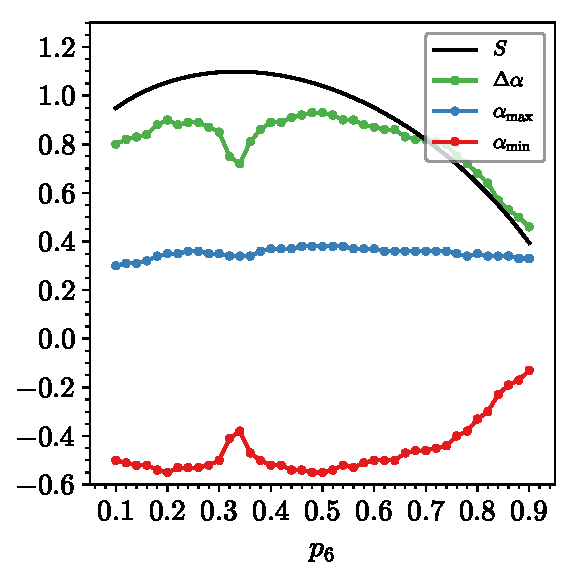
\includegraphics[width=7cm]{./figures/targeted_opt/topt_alpha_limits.pdf}
	\caption{Accessible range of the \aw{} parameter in the aG system.%, for variable $p_6$.}
	}
	\label{fig:alphalim}
\end{figure}


\subsection{Structure and Energetics}

To explore the structural properties of the aG networks at different values of $p_6$ and $\alpha$, 100 periodic networks containing $10^5$ rings, were constructed for $p_6=0.2,0.4,0.6,0.8$. 
These simulations were performed with geometry optimisation and so also provide information on the physical limits on $\alpha$.
Figure \ref{fig:toptenergy1} displays the mean and standard deviation of the total potential energy for each $p_6$ atomic network across a range of $\alpha$ values. 
It can be seen that the energy minimum in each case is only weakly dependent on the value of $p_6$, varying from $\alpha\simeq{0.23}$ at $p_6=0.8$ to $\alpha\simeq{0.27}$ at $p_6=0.2$, and close to the value of $\alpha$ seen across many natural systems. 
Whilst there is little cost for small deviations from the minimum, decreasing $\alpha$ rapidly incurs a relatively large energetic penalty. 
Figure \ref{fig:toptenergy2} shows the analogous energies when minimising through the dual lattice alone. 
The curves have a very similar form with the minima aligned, suggesting that working in dual space can be sufficient to capture all system properties, with a much lower computational overhead.

%The overall energetic ordering of the different systems is also reflective of underlying ring structure.
%As is intuitive, the greater the number of $5$\-- and $7$\-- rings in the aG system the higher the energy minimum.
%The energy is not necessarily a solely a function of the range of accessible rings.
%The structures based on the \zach{} statistics are always higher in energy than those with the silica distribution, despite the silica samples containing larger rings.
%This is a manifestation of the \zach{} networks being inherently more ``unphysical'' as previously discussed.

\begin{figure}[bt]
     \centering
     
     \begin{subfigure}[b]{0.45\textwidth}
         \centering
         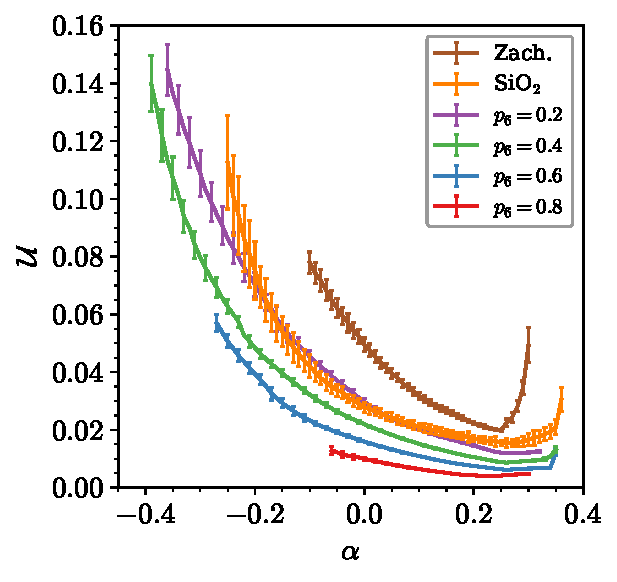
\includegraphics[width=\textwidth]{./figures/targeted_opt/topt_u_graph.pdf}
         \caption{}%Minimisation through atomic network}
         \label{fig:toptenergy1}
     \end{subfigure}
     \hfill
	\begin{subfigure}[b]{0.45\textwidth}
         \centering
         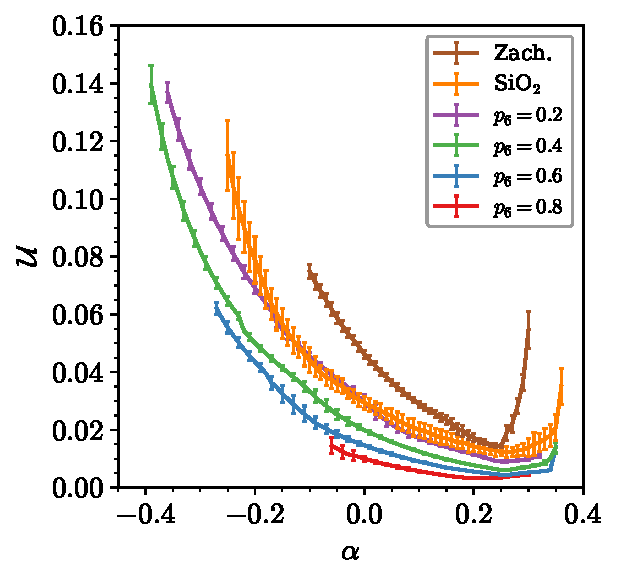
\includegraphics[width=\textwidth]{./figures/targeted_opt/topt_u_dual.pdf}
         \caption{}%Minimisation through ring network}
         \label{fig:toptenergy2}
     \end{subfigure}

     \caption{Geometry optimised potential energy of configurations produced via targeted optimisation for a range of systems with variable $\alpha$ parameter, with bars indicating one standard deviation from the mean. Panel (a) gives the results of optimisation through the atomic network with the Keating potential, whilst panel (b) gives the optimisation through the ring network with a simple harmonic potential.}
     \label{fig:toptenergy}
\end{figure}

Partial radial distribution functions (RDFs) can be used to further quantify any ordering imposed on the generated configurations (see section \ref{s:rdfs}).
These partial RDFs are constructed in reference to the distance of the centroids of a $k$\--ring from a central $j$\--ring, denoted $g_{jk}\left(r\right)$.
They can therefore equivalently be thought of as the dual space RDFs between nodes of degrees $j,k$.
The Euclidean distance is used as opposed to the topological distance (\ie{} the number of links from a given node) as the latter has been shown to lead to artificial long range correlations \cite{Sadjadi2016}. 

Figures \ref{fig:toptrdf1} and \ref{fig:toptrdf2} show the partial RDFs for the 5\--5 and 5\--7 ring pairings, $g_{55}\left(r\right)$ and $g_{57}\left(r\right)$ respectively.
As is consistent with its intuitive meaning, increasing $\alpha$ causes a reduction in intensity in the first peak of $g_{55}\left(r\right)$ and a concomitant increase in intensity in the first peak of $g_{57}\left(r\right)$, as 5\--5 adjacencies are replaced with 5\--7. 
In addition, the position of the first peak shifts to smaller $r$ as $\alpha$ is reduced, reflecting both the increased distortion in the rings and the deviation from the ideal $120^\circ$ bond angle, which translates to the higher observed potential energy.

\begin{figure}[bt]
     \centering
     
     \begin{subfigure}[b]{0.45\textwidth}
         \centering
         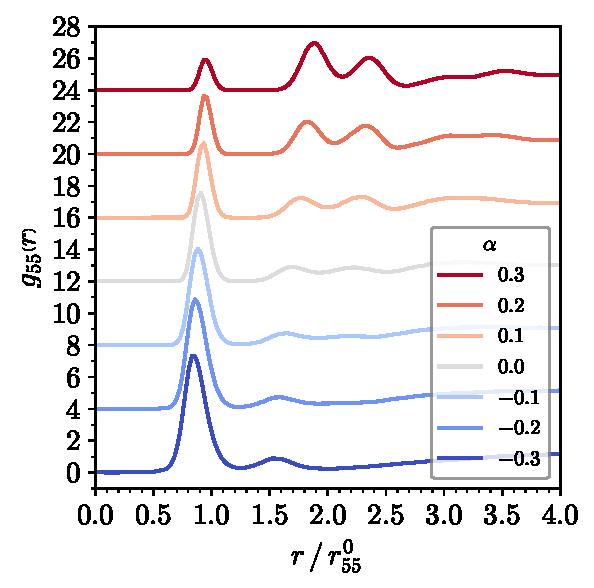
\includegraphics[width=\textwidth]{./figures/targeted_opt/partial_gr_55_567.pdf}
         \caption{}
         \label{fig:toptrdf1}
     \end{subfigure}
     \hfill
     \begin{subfigure}[b]{0.45\textwidth}
         \centering
         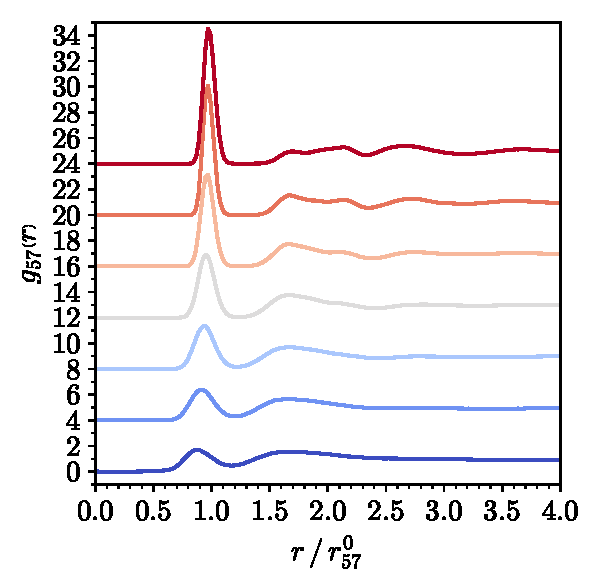
\includegraphics[width=\textwidth]{./figures/targeted_opt/partial_gr_57_567.pdf}
         \caption{}
         \label{fig:toptrdf2}
     \end{subfigure}
     
     \vspace{2mm}
     \begin{subfigure}[b]{0.45\textwidth}
         \centering
         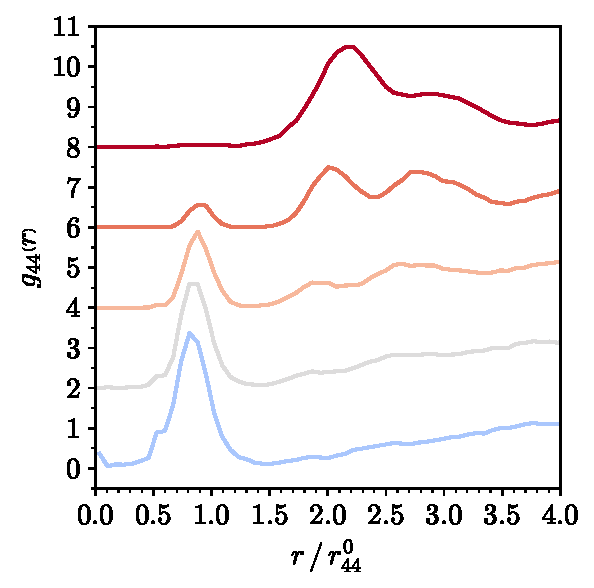
\includegraphics[width=\textwidth]{./figures/targeted_opt/partial_gr_44_zach.pdf}
         \caption{}
         \label{fig:toptrdf3}
     \end{subfigure}
     \hfill
     \begin{subfigure}[b]{0.45\textwidth}
         \centering
         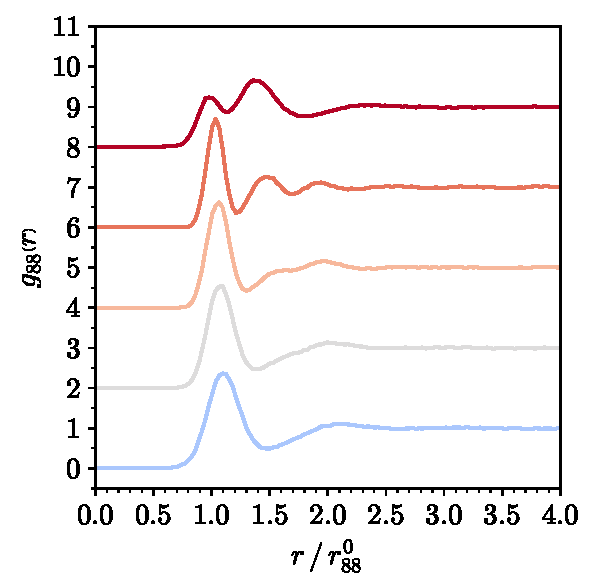
\includegraphics[width=\textwidth]{./figures/targeted_opt/partial_gr_88_zach.pdf}
         \caption{}
         \label{fig:toptrdf4}
     \end{subfigure}
     
     \caption{Partial RDFs for the aG (panels (a)\--(b)) and \zach{} (panels (c)\--(d)) systems illustrate the evolution in ring structure with varying $\alpha$ parameter.}
     \label{fig:toptrdf}
\end{figure}

These figures also show significant structural evolution beyond the nearest-neighbour length scale. 
As $\alpha$ becomes more positive, peaks emerge in $g_{55}\left(r\right)$ at $r/r_{55}^0\approx{1.8}$ and $\approx{2.3}$. 
An increase in $\alpha$ corresponds to a greater tendency for 7\--rings to
be near\--neighbours to 5\--rings and, in turn, increases the probability of the same 7\--ring having a second 5\--ring near\--neighbour. 
In simple geometric terms, the second 5\--ring can occupy three possible sites around the 7\--ring, the non\--adjacent positions corresponding to the developing peaks. 
Note that one might na\"ively assume that driving $\alpha$ to more positive values would tend to eliminate the nearest-neighbour 5\--5 spatial correlations. However, figure \ref{fig:toptrdf1} indicates this not to be the case, reflecting the balance between retaining these units and facilitating nearest\--neighbour 5\--7 ring interactions via the formation of 5\--7\--5 triplets.

Similar analysis was performed on 100 generated \zach{} and \sioii{} networks.
Although the algorithm requires the fit to equation \eqref{eq:aboavweaire} to be exactly linear for the aG system, for broader ring distributions this is no longer the case. 
However, for the \zach{} configuration the linear regression ($R^2$) coefficient was always in excess of $0.995$, and for the silica the average $R^{2}$ was $0.979$, representing a very good fit. 
Figure \ref{fig:toptenergy1} shows the energies of both the \zach{} and \sioii{} systems as a function of $\alpha$. 
Both cases resemble those for the aG with energy minima at $\alpha\approx{0.25}$. The silica curve shows smaller curvature reflecting the broader distribution
of ring sizes whilst the \zach{} curve shows a greater curvature reflecting the ``extreme'' (\ie{} physically unrealistic) nature of the distribution.
In addition it proved difficult to generate low $\alpha$ configurations ($\alpha<-0.1$) for the Zachariasen network.

Figures \ref{fig:toptrdf3} and \ref{fig:toptrdf4} show two key RDFs for the \zach{} configuration, $g_{44}\left(r\right)$ and $g_{88}\left(r\right)$, highlighting the spatial correlations between the smallest and largest rings in the system. 
The effects of changing $\alpha$ on $g_{44}\left(r\right)$ are dramatic with strong nearest\--neighbour clustering at negative values. 
In this case, however, the nearest-neighbour 4-4 correlations do vanish at high $\alpha$ as 4\--8 nearest\--neighbour correlations dominate but the 8\--ring is large enough to accommodate up to four 4\--ring nearest\--neighbours without any 4\--4 neighbouring pairs. 
Again this is demonstrated through the next nearest neighbours by the 8\--4\--8 peak developing at $r/r_{88}^0\approx 1.4$.


\section{Ring Percolation in Amorphous Graphene}

As a further demonstration of the utility and scope of the targeted optimisation algorithm, a short study is presented on the percolation of different ring sizes in aG systems.
Owing to the fact that this is a standalone section, the theory pertinent to this investigation is first presented, followed by results.

\subsection{Percolation Theory and Clustering}
\label{s:percolationtheory}

Percolation theory has its roots in problems concerning the flow of fluids through porous media \cite{Broadbent1956}, but now it can more generally be thought of as relating to the connectedness of components in a network (also referred to as \textit{robustness}) \cite{Callaway2000}.
The theory of clustering and percolation is an extremely rich field, which this thesis will merely dip its toe into, and so the discussion of the underlying theory is framed in the context of the aG networks already introduced in this chapter.

As an introductory example, consider a pristine hexagonal lattice for which the dual structure is a triangular net.
It is clear that in this lattice all the nodes are connected \ie{} there is some continuous path linking any two given rings.
Equally, one could say that all the rings belong to the same cluster.
Now imagine the process of removing nodes sequentially and at random from the original lattice, as shown in figure \ref{fig:perctri}.
Initially, removing nodes will have little effect on the network structure, but after a sufficient number are deleted, the interconnectivity of all the nodes will likely be broken, and the original large cluster will fragment into smaller clusters.
At some point, the lattice will undergo a phase transition, from one in which there is a single ``giant'' component to one which has many small components.
Quantifying this behaviour is the essence of percolation theory \-- exploring this transition and determining at what point this ``percolation threshold'' occurs.

\begin{figure}[bt]
     \centering
         
     \begin{subfigure}[b]{0.3\textwidth}
         \centering
         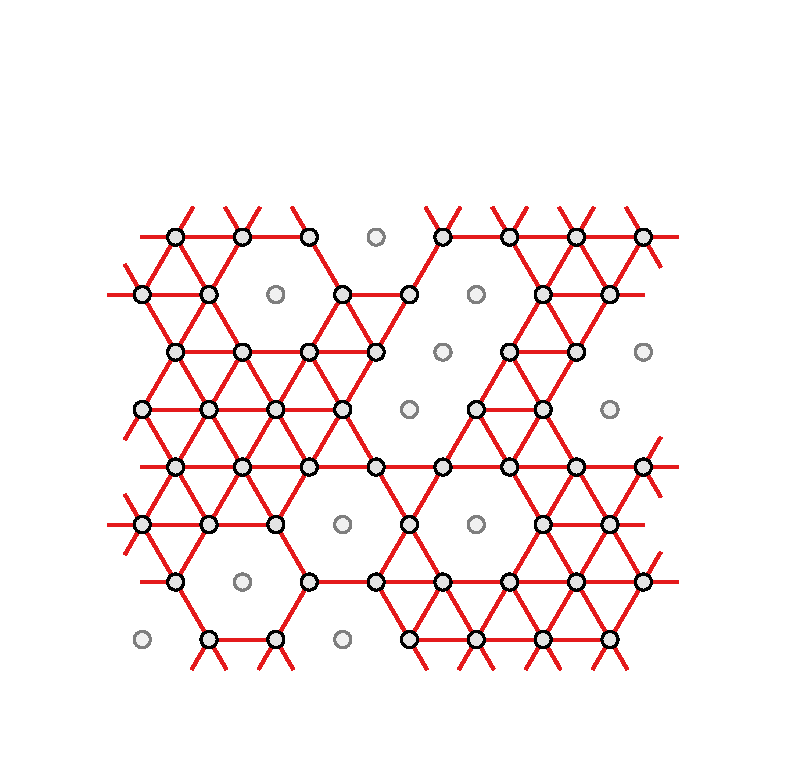
\includegraphics[width=\textwidth]{./figures/targeted_opt/perc_tri_8.pdf}
         \caption{$p=0.8$}
         \label{fig:perctri8}
     \end{subfigure}
     \hfill
      \begin{subfigure}[b]{0.3\textwidth}
         \centering
         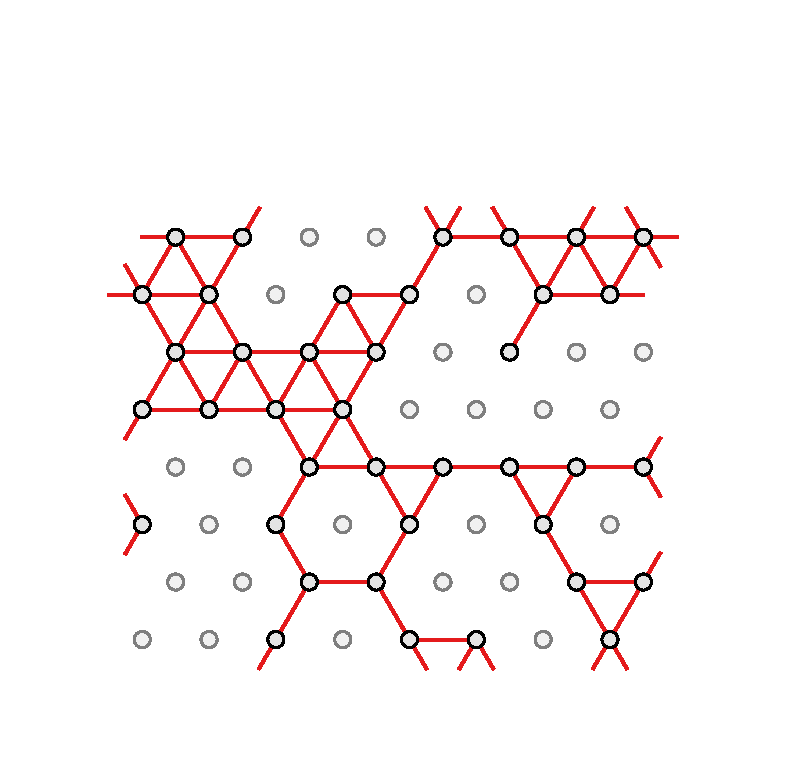
\includegraphics[width=\textwidth]{./figures/targeted_opt/perc_tri_6.pdf}
         \caption{$p=0.6$}
         \label{fig:perctri6}
     \end{subfigure}
     \hfill
      \begin{subfigure}[b]{0.3\textwidth}
         \centering
         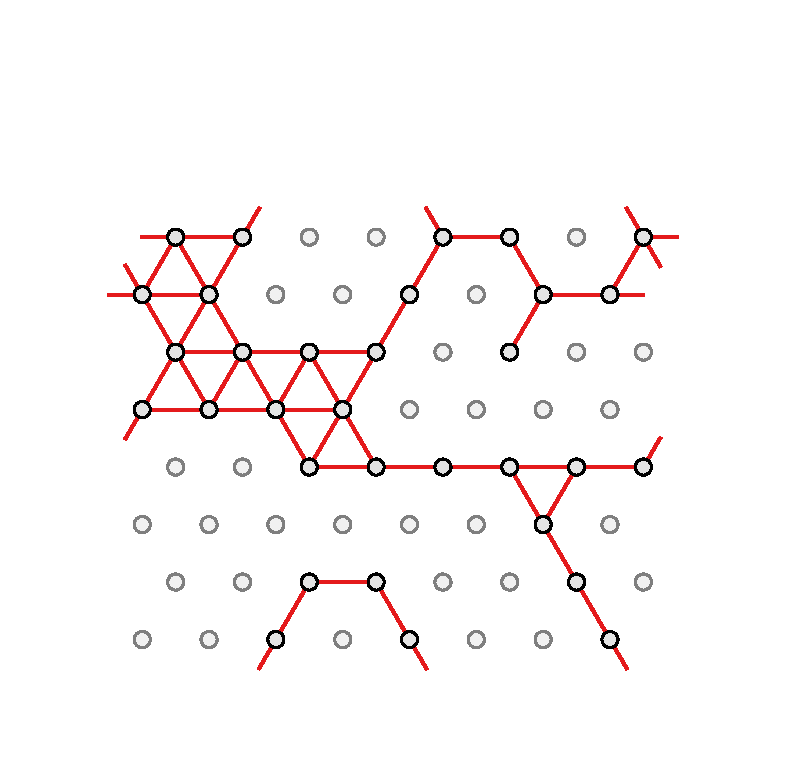
\includegraphics[width=\textwidth]{./figures/targeted_opt/perc_tri_5.pdf}
         \caption{$p=0.5$}
         \label{fig:perctri5}
     \end{subfigure}
     \hfill
     
     \vspace{0.2cm}
          \begin{subfigure}[b]{0.3\textwidth}
         \centering
         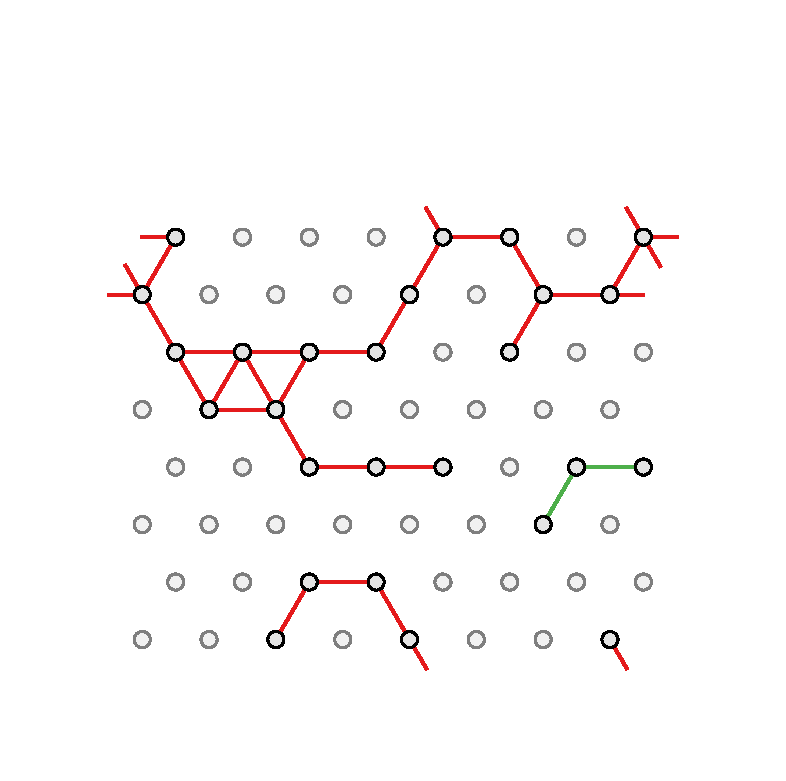
\includegraphics[width=\textwidth]{./figures/targeted_opt/perc_tri_4.pdf}
         \caption{$p=0.4$}
         \label{fig:perctri4}
     \end{subfigure}
     \hfill
      \begin{subfigure}[b]{0.3\textwidth}
         \centering
         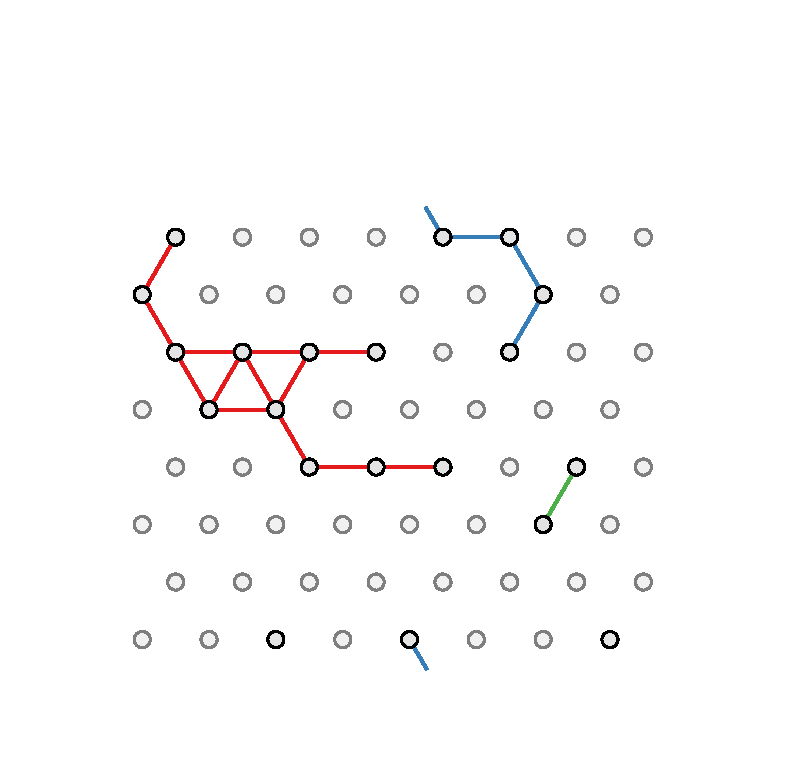
\includegraphics[width=\textwidth]{./figures/targeted_opt/perc_tri_3.pdf}
         \caption{$p=0.3$}
         \label{fig:perctri3}
     \end{subfigure}
     \hfill
         \begin{subfigure}[b]{0.3\textwidth}
         \centering
         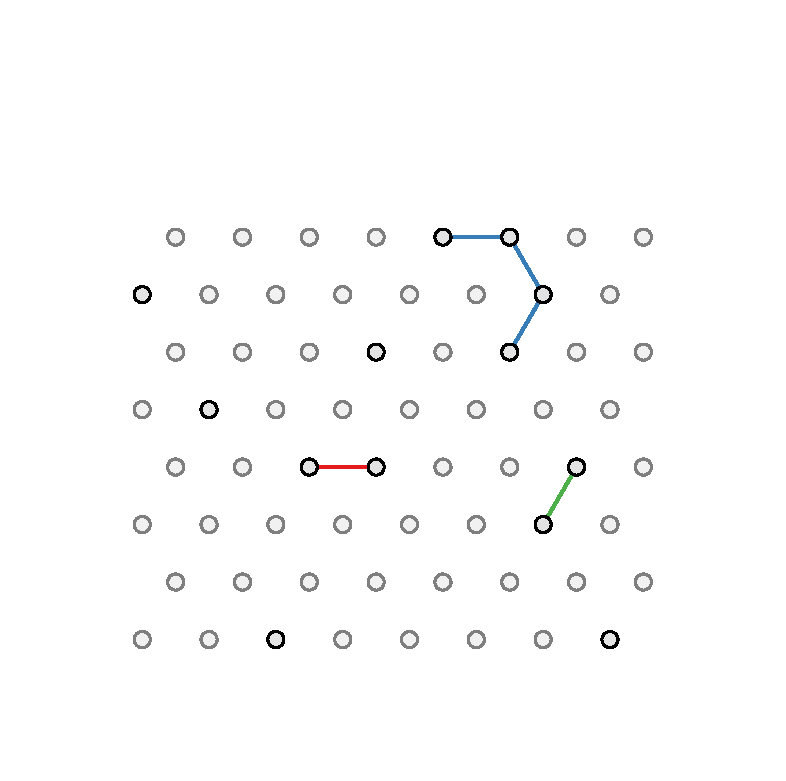
\includegraphics[width=\textwidth]{./figures/targeted_opt/perc_tri_2.pdf}
         \caption{$p=0.2$}
         \label{fig:perctri2}
     \end{subfigure}
     \hfill
     
     \caption{Site percolation on a triangular lattice. Panels (a)\--(f) show network structure as site occupancy is decreased, as indicated in the captions. Full circles signify occupied sites whilst connections are given by coloured lines, with the colour indicating nodes forming part of the same cluster.}
     \label{fig:perctri}
\end{figure}

To formalise this slightly, take an infinite triangular lattice, of which a random proportion, $p$, of nodes are occupied.
The size of a cluster (\ie{} the number of nodes which comprise it) can be denoted, $s$. 
The probability of a node belonging to a cluster of size $s$ is then $P_s$, and so the probability of belonging to an infinitely sized cluster $P_{\infty}$ \cite{StaufferDietrich2014}.
The percolation threshold, $p_c$, is then the critical occupancy at which a giant component appears \ie{}
\begin{equation}
	P_{\infty}=\begin{cases} 1 \quad p\geq p_c \\
							0 \quad p<p_c
	\end{cases}.
\end{equation}
Additionally, at this critical point, measures such as the average finite cluster size and connectedness length diverge.
For the example given above, which is the classic example of site percolation on a triangular lattice, the percolation threshold is $p_c=\frac{1}{2}$  \cite{Sykes1964}.

The case of the triangular lattice above is one of the few examples of problems in percolation theory that can be solved analytically \cite{Kirkpatrick1973}.
In order to find percolation thresholds for all but the simplest cases, numerical methods must be used.
This problem is an ideal candidate for solution using a \mc{} method \cite{Frisch1962,Dean1967}.
One potential concern with a numerical method is that the lattices involved must be finite.
The solution is to approximate the probability of a node residing in the infinite cluster as the probability of a node residing in the largest cluster. 
This is to say, if there are $N$ nodes in the lattice and the maximum lattice size is $s_{\text{max}}$, then
\begin{equation}
	P_{\infty}\approx \frac{s_\text{max}}{N}\,.
\end{equation} 
This expression will hold in the limit of $N\rightarrow \infty$.
As will be seen in section \ref{s:percphasediagram}, for finite size lattices this approximation leads to smoothing of the step\--like form of $P_{\infty}$.
The percolation threshold in this case is then approximated by as the occupancy, $p$, for which $P_{\infty}=\frac{1}{2}$.

\subsection{Percolation in Disordered Networks}

\begin{figure}[bt]
     \centering
     
     \begin{subfigure}[b]{0.3\textwidth}
         \centering
         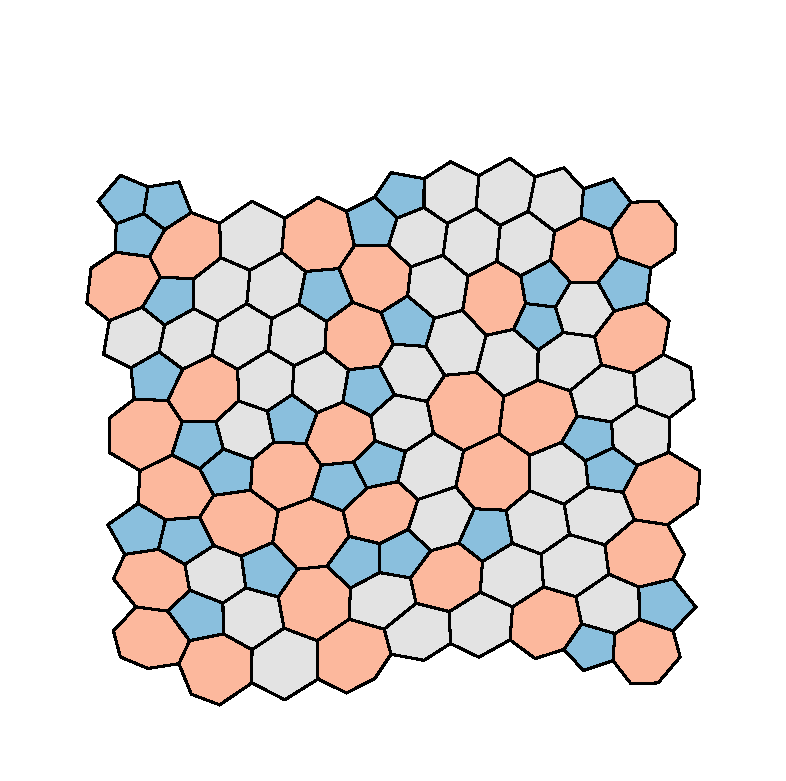
\includegraphics[width=\textwidth]{./figures/targeted_opt/subgraph_rings.pdf}
         \caption{Ring structure}
         \label{fig:percsub1}
     \end{subfigure}
     \hspace{1cm}
      \begin{subfigure}[b]{0.3\textwidth}
         \centering
         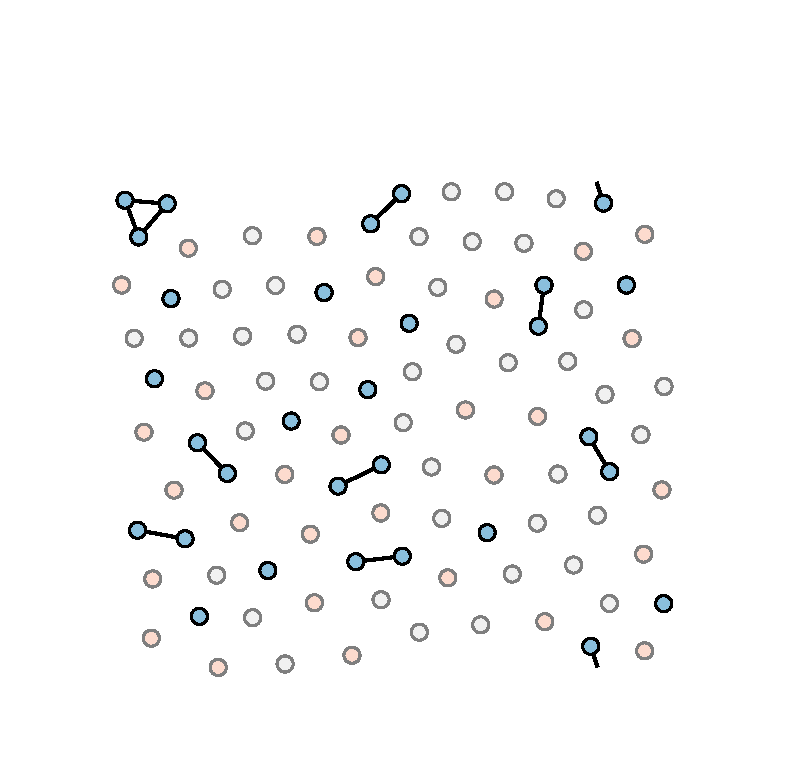
\includegraphics[width=\textwidth]{./figures/targeted_opt/subgraph_5.pdf}
         \caption{5\--ring subgraph}
         \label{fig:percsub2}
     \end{subfigure}
     
     \vspace{0.2cm}
      \begin{subfigure}[b]{0.3\textwidth}
         \centering
         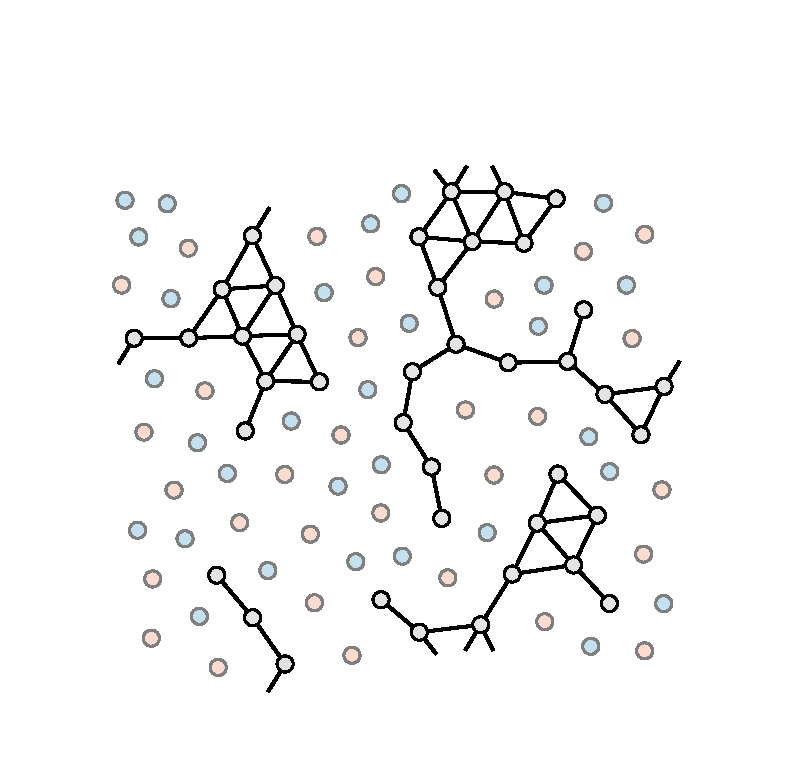
\includegraphics[width=\textwidth]{./figures/targeted_opt/subgraph_6.pdf}
         \caption{6\--ring subgraph}
         \label{fig:percsub3}
     \end{subfigure}
     \hspace{1cm}
     \begin{subfigure}[b]{0.3\textwidth}
         \centering
         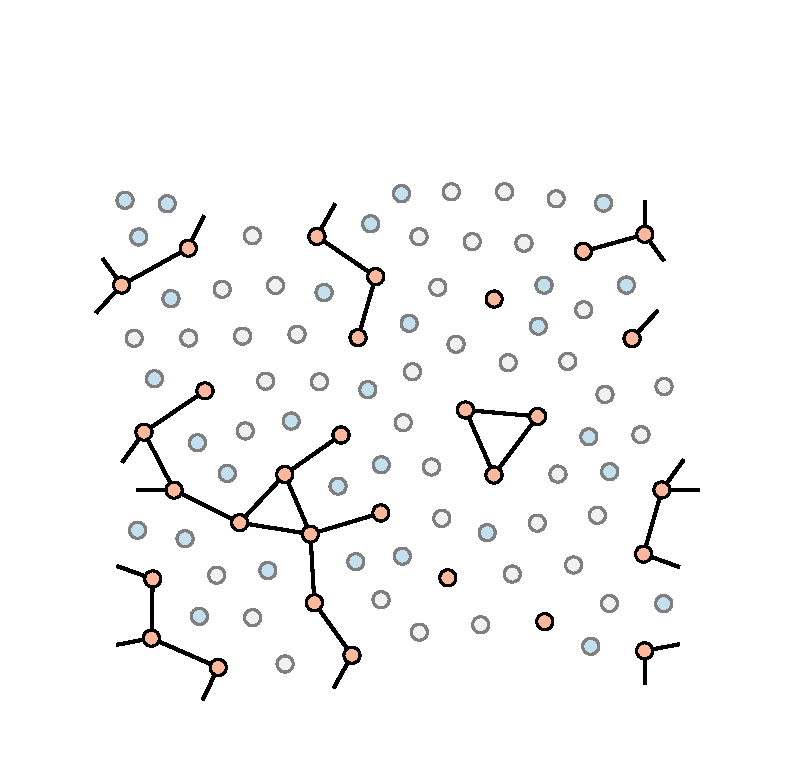
\includegraphics[width=\textwidth]{./figures/targeted_opt/subgraph_7.pdf}
         \caption{7\--ring subgraph}
         \label{fig:percsub4}
     \end{subfigure}
     
     \caption{Panel (a) gives an example disordered aG ring structure and panels (b)\--(d) the associated $k$\--ring subgraphs, as indicated in the figure captions. Each subgraph contains only vertices and edges pertaining to the given ring size.}
     \label{fig:subgraphs}
\end{figure}

The example in the preceding section concerns site percolation on a regular lattice, where each site is equivalent.
However, the ring networks of interest in this work are disordered, where sites have different degrees (reflecting ring sizes).
Disordered lattices therefore have an extra degree of complexity when compared to their ordered analogues.
This raises the possibility of studying the percolation of different ring sizes in the network.
To achieve this, one must first construct the subgraphs for each ring size, which contain only the vertices and edges which relate to a given node degree, as shown  in figure \ref{fig:subgraphs}.
The percolation threshold can then be studied for each of these subgraphs.
For each $k$\--ring subgraph, the percolation threshold will naturally depend on the global ring statistics, $p_k$.
However, unlike the regular lattices, the percolation threshold must also depend on the ring correlations, which must influence the clustering \cite{Newman2003}.
As seen throughout this chapter, this property is controllable through the \aw{} parameter.
Therefore, for each $k$\--ring subgraph, the percolation threshold will be a function of both a critical ring frequency, $p_k^c$, and a critical \aw{} value $\alpha_k^c$.

\subsection{Percolation Phase Diagram of Amorphous Graphene}
\label{s:percphasediagram}

The percolation phase behaviour was investigated for the aG system, containing only 5\--, 6\-- and 7\--rings.
Again this system is relatively well defined in terms of the ring statistics, as shown by equation \ref{eq:agcon}.
As the accuracy of the percolation transition is dependent on the system size, very large networks were generated with $1\times10^6$ rings.
This remained computationally tractable as the calculation of percolation requires only the node connectivities, not their positions, and so there is no need for geometry optimisation.
Networks were constructed using targeted optimisation across the full spectrum of $p_6$ values and with $\alpha$ in the range $-0.1\rightarrow 0.3$.
For each state point, $100$ networks were sampled starting from different random seeds. 

\begin{figure}[bt]
     \centering
     
     \begin{subfigure}[b]{0.45\textwidth}
         \centering
         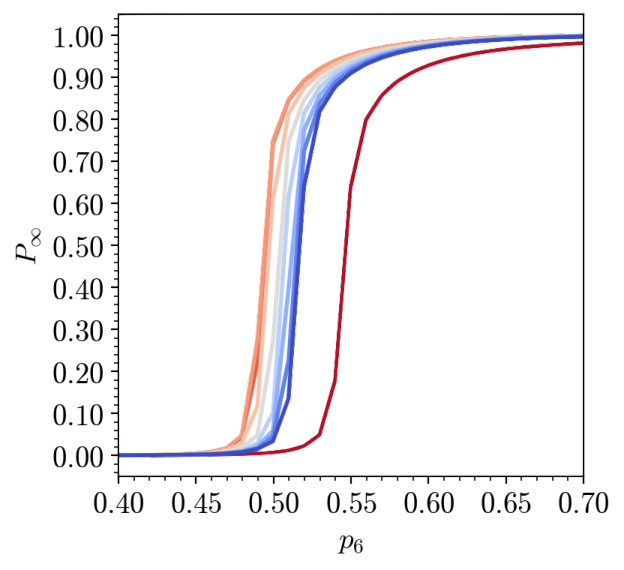
\includegraphics[width=\textwidth]{./figures/targeted_opt/perc1.pdf}
         \caption{}
         \label{fig:percres1}
     \end{subfigure}
     \hfill
      \begin{subfigure}[b]{0.45\textwidth}
         \centering
         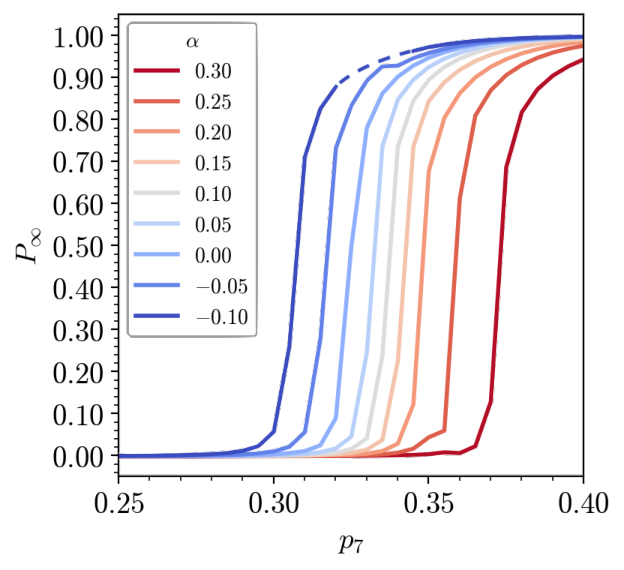
\includegraphics[width=\textwidth]{./figures/targeted_opt/perc2.pdf}
         \caption{}
         \label{fig:percres2}
     \end{subfigure}
     \hfill
     
      \begin{subfigure}[b]{0.5\textwidth}
         \centering
         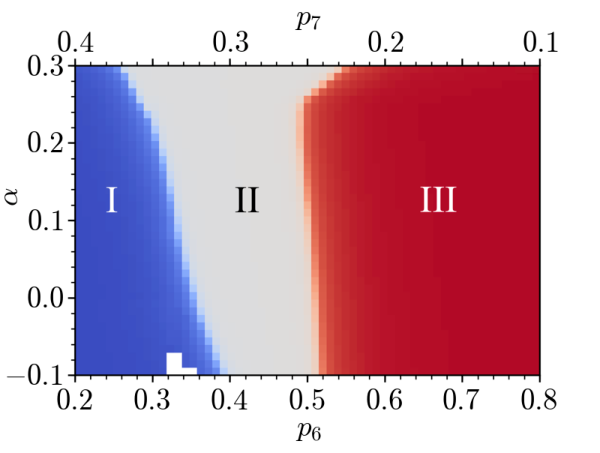
\includegraphics[width=\textwidth]{./figures/targeted_opt/perc3.pdf}
         \caption{}
         \label{fig:percres3}
     \end{subfigure}
     \hfill
     
     \caption{Percolation in aG configurations generated via targeted optimisation. Panels (a) and (b) map percolation as a function of $\alpha$ and $p_6$, $p_7$ respectively (dashed line indicates interpolated data, both share the same legend). The percolation threshold is defined as when $P_\infty=\frac{1}{2}$. Panel (c) gives the phase behaviour of these systems: phase I (blue area) contains a giant component in the 7\--ring subgraph; phase II (grey area) no giant components in any subgraph; phase III (red area) a giant component in the 6\--ring subgraph.}
     \label{fig:percolationres}
\end{figure}

The results of these simulations are presented in figure \ref{fig:percolationres}.
Figures \ref{fig:percres1} and \ref{fig:percres2} show the evolution in $P_\infty$ for selected $\alpha$ values across the $p_k$ range for the 6\-- and 7\--ring subgraphs, which demonstrate slightly different behaviours.
Neglecting the effect of the \aw{} parameter initially, as the proportion of a given ring increases, the probability of a giant component forming increases.
This is process is visualised in figures \ref{fig:percp7a}\--\ref{fig:percp7c}.
In the case of the 6\--ring subgraph, there is similarity to the triangular site percolation problem discussed in section \ref{s:percolationtheory}, with the percolation threshold oscillating around $p_6^c\approx0.5$.
The 7\--ring case on the other hand displays a percolation threshold at a lower value of $p_7^c\approx0.35$.
This is intuitive as each node has a greater number of edges emanating from it, and so a greater probability of connecting to other rings.
It is also for this reason that there is \textit{no} percolation threshold for the 5\--ring subgraph in aG.
This can be rationalised by realising that as $p_5=p_7$, and a 7\--ring by definition has more connections to adjacent rings than the 5\--ring, there can never be a point where the 5\--rings can form a giant component in preference to the 7\--rings.
In the most extreme case, one can see this in the example of haeckelite, in which $p_5=p_7=\frac{1}{2}$ and all 7\--rings are connected, yet the 5\--rings remain isolated from one another.

\begin{figure}[bt]
     \centering
     
     \begin{subfigure}[b]{0.3\textwidth}
         \centering
         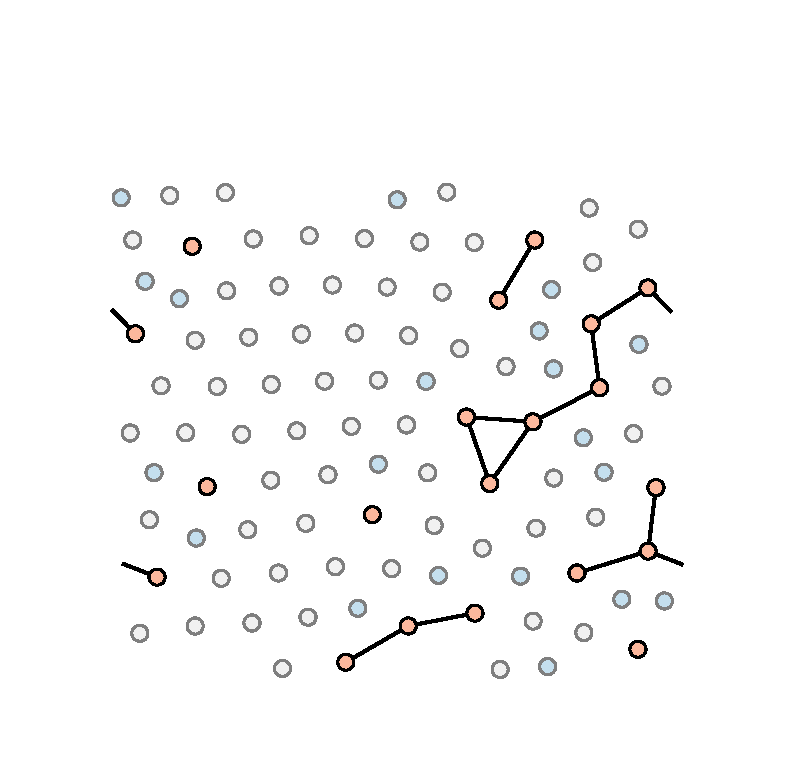
\includegraphics[width=\textwidth]{./figures/targeted_opt/percolation_p7_2.pdf}
         \caption{$p_7=0.2$, $\alpha\approx0.25$}
         \label{fig:percp7a}
     \end{subfigure}
     \hfill
      \begin{subfigure}[b]{0.3\textwidth}
         \centering
         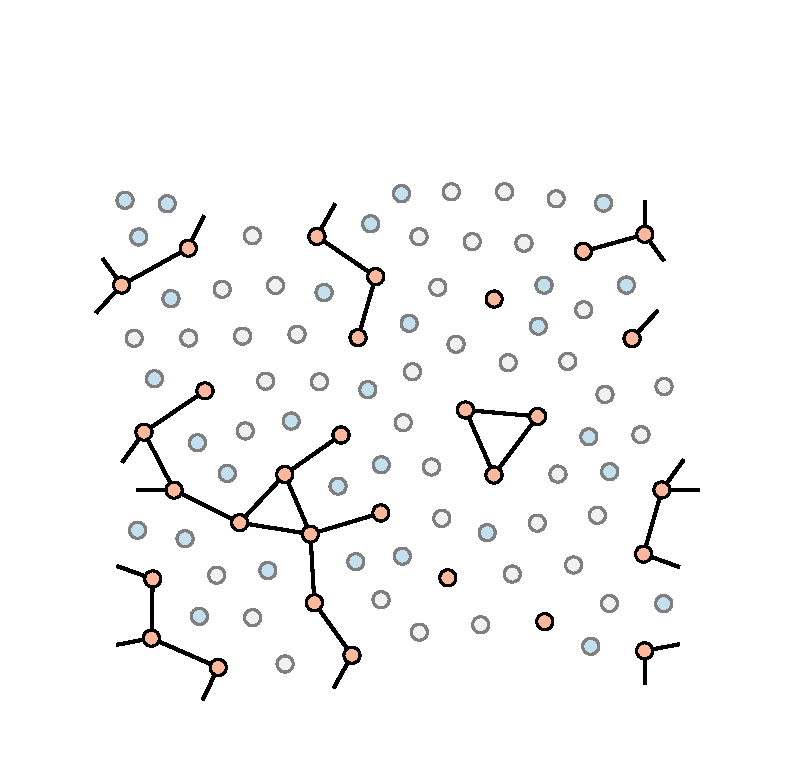
\includegraphics[width=\textwidth]{./figures/targeted_opt/percolation_p7_3.pdf}
         \caption{$p_7=0.3$, $\alpha\approx0.25$}
         \label{fig:percp7b}
     \end{subfigure}
     \hfill
      \begin{subfigure}[b]{0.3\textwidth}
         \centering
         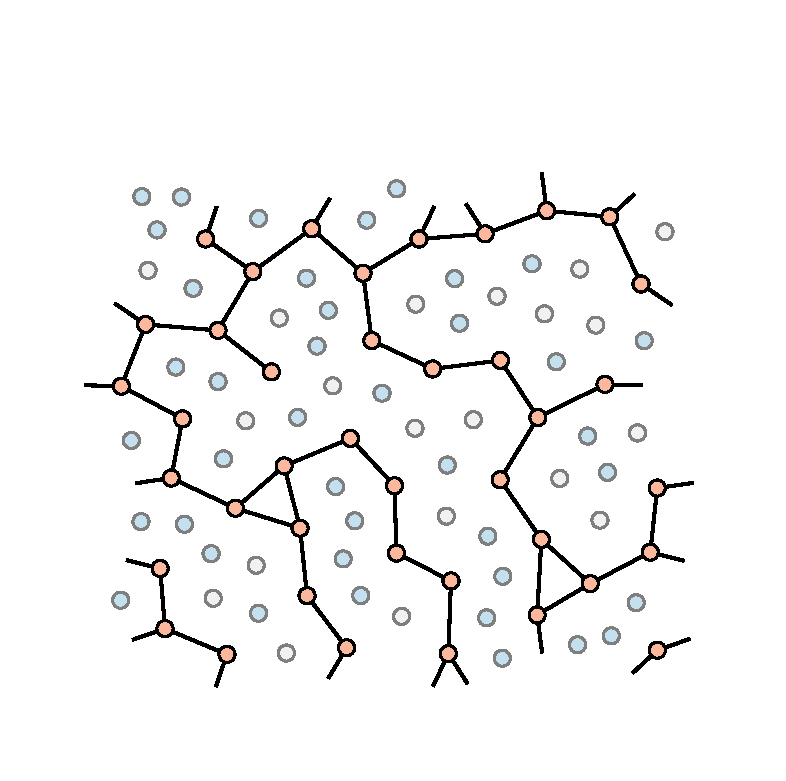
\includegraphics[width=\textwidth]{./figures/targeted_opt/percolation_p7_4.pdf}
         \caption{$p_7=0.4$, $\alpha\approx0.25$}
         \label{fig:percp7c}
     \end{subfigure}
     
     \vspace{0.2cm}
     \begin{subfigure}[b]{0.3\textwidth}
         \centering
         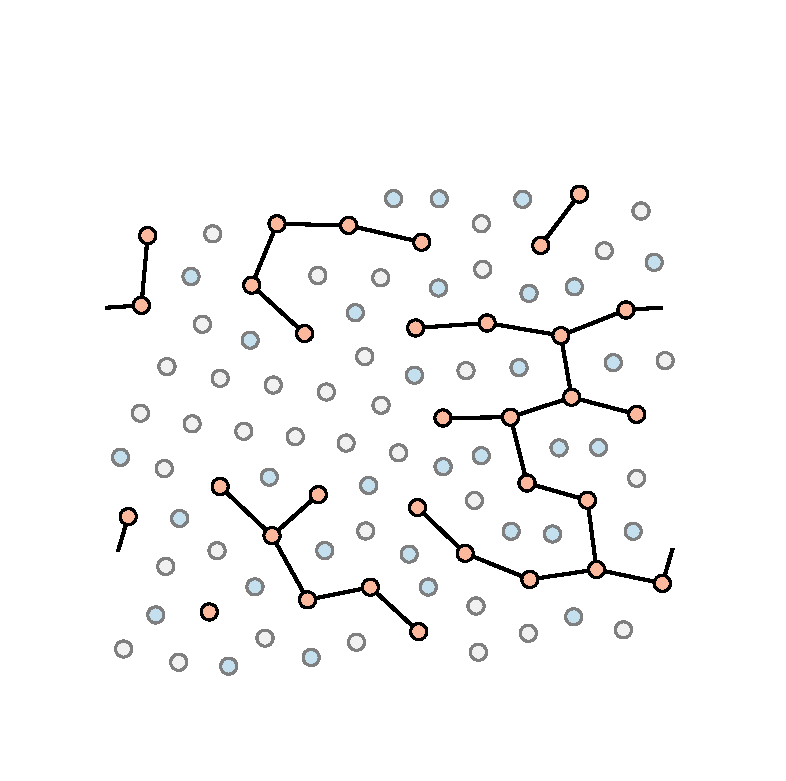
\includegraphics[width=\textwidth]{./figures/targeted_opt/percolation_alpha_3.pdf}
         \caption{$p_7=0.32$, $\alpha\approx0.3$}
         \label{fig:percalphaa}
     \end{subfigure}
     \hfill
      \begin{subfigure}[b]{0.3\textwidth}
         \centering
         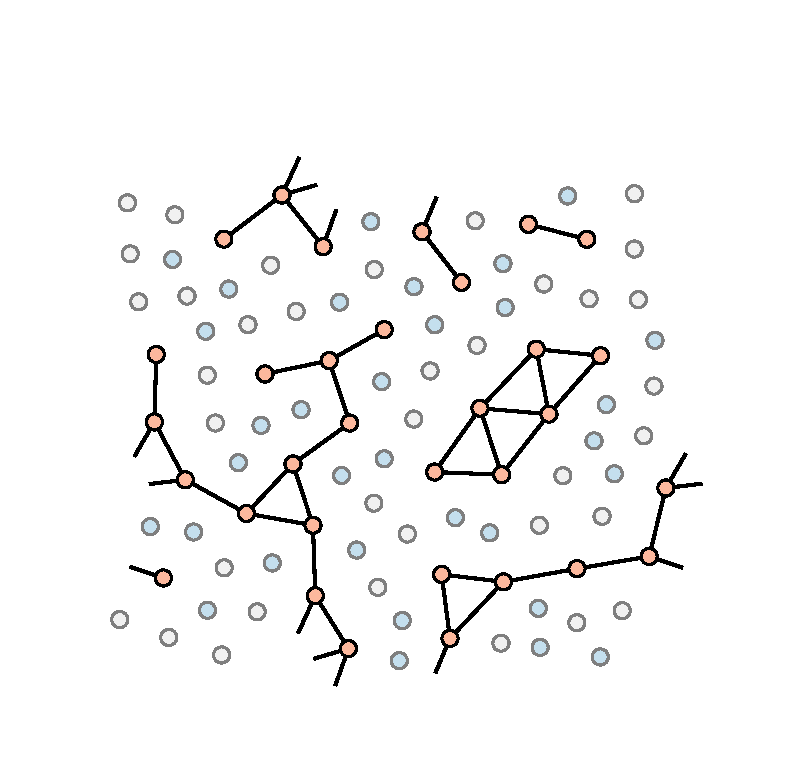
\includegraphics[width=\textwidth]{./figures/targeted_opt/percolation_alpha_1.pdf}
         \caption{$p_7=0.32$, $\alpha\approx0.1$}
         \label{fig:percalphab}
     \end{subfigure}
     \hfill
      \begin{subfigure}[b]{0.3\textwidth}
         \centering
         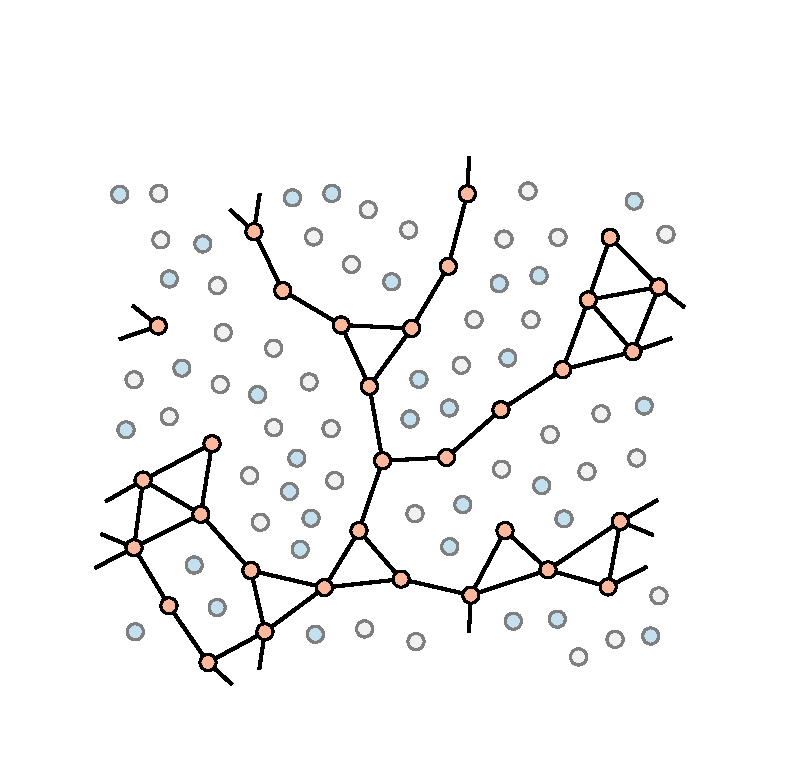
\includegraphics[width=\textwidth]{./figures/targeted_opt/percolation_alpha_-1.pdf}
         \caption{$p_7=0.32$, $\alpha\approx-0.1$}
         \label{fig:percalphac}
     \end{subfigure}
     \hfill
     
     \caption{The formation of giant components in disordered networks is a function of both the proportion of each ring size (here $p_7$) and the ring correlations (as measured by $\alpha$). Panels (a)\--(c) show the effect of increasing $p_7$ at constant $\alpha$, with a giant component only forming in (c), once a sufficient number of 7\--rings are present. Conversely panels (d)\--(f) show the effect of decreasing $\alpha$ at constant $p_7$, with a giant component only forming in (f), once sufficient clustering of 7\--rings is achieved.}
     \label{fig:percolationag}
\end{figure}

The behaviour of the network percolation threshold is also subtly related to the node correlations, as expected \cite{Zhou2012,Schmeltzer2014}.
For the 7\--ring subgraph, the percolation threshold in $p_7$ systematically decreases with decreasing $\alpha$.
This is because a decreasing $\alpha$ is reflective of increased large\--large ring pairings, thus facilitating the formation of a giant connected  component of 7\--rings.
This process is demonstrated in figures \ref{fig:percalphaa}\--\ref{fig:percalphac}.
The 6\--ring shows what appears to be a more complex relationship with $\alpha$.
Initially as $\alpha$ is increased, the percolation threshold in $p_6$ decreases, before suddenly increasing again at high $\alpha$.
This is a consequence of the fact that the 6\--ring is the ``middle'' ring size. 
Hence when $\alpha$ is strongly negative, 7\--6 pairings are most favoured and when $\alpha$ is strongly positive 6\--5 pairings are more abundant.
It is only when $\alpha$ sits in the intermediate region that the 6\--6 ring correlations are maximised and percolation is most readily facilitated.
It is interesting to note that this also around the value of $\alpha\approx 0.25$ that is also common in nature.

The results discussed above can be combined to draw a percolation phase diagram for aG, presented in figure \ref{fig:percres3}.
In this diagram there are three phases:
\begin{itemize}
	\item \textbf{Phase I}: exists at $p_6\lesssim 0.35$ and preferentially at low $\alpha$, where networks contain a giant component of 7\--rings
	\item \textbf{Phase II}: occupies intermediate values of $p_6$, where no subgraph contains a giant component
	\item \textbf{Phase III}: encompasses the largest region of phase space, for $p_6\gtrsim0.5$, where networks contain a giant component of 6\--rings
\end{itemize}
From this phase behaviour it is evident that relatively low values of $p_6$ must be achieved before the percolation of 6\--rings is broken.
In addition it is unlikely that phase I could be experimentally realised and percolation of the 7\--rings achieved. 
This is because from maximum entropy, the most disordered lattice possible would have $p_5=p_6=p_7=\frac{1}{3}$ which is on the fringe of the percolation threshold for $p_7$, and would necessitate a value of $\alpha$ much lower than is currently seen experimentally.
This could have implications when designing materials, for which there are eigenstates localised on specific ring sizes \cite{Kapko2010,Zhu2016}.




\section{Chapter Conclusions}

An novel method has been presented to generate \td{} network materials with well defined topology. 
This targeted \mc{} search algorithm allows configurations to be constructed which have precise ring size distributions and ring\--ring correlations.
The advantage of this approach is that configurations can be produced rapidly with controllable properties; which may lie outside experimentally or physically accessible regions of phase space.
These configurations may then be used as starting points for further investigations.
For example, the algorithm outlined in this work has already been utilised to study the mechanical properties of vitreous silica under deformation \cite{Bamer2020,Ebrahem2020a}.

In this chapter the targeted optimisation method was employed to probe the physical meaning of the \aw{} parameter.
The effect of $\alpha$ on the ring structure has been quantified through partial RDFs, and the energetic minima for a range of systems has been shown to correspond well with values commonly found in nature.
Finally, the method was used in a study of the ring percolation in amorphous graphene, with the phase behaviour quantified in terms of the ring statistics and \aw{} parameter.

 





